\documentclass[12pt, a4paper]{article}
\usepackage[utf8]{inputenc}
\usepackage{polski}
\usepackage{amssymb}
\usepackage{amsmath}
\usepackage{fancyhdr}
\usepackage{multicol}
\usepackage{graphicx}
\setlength{\voffset}{-0.75in}
\setlength{\headsep}{5pt}
\setlength{\hoffset}{-40pt}
\setlength{\textwidth}{500pt}
\setlength{\textheight}{770pt}
\setlength{\parindent}{0em}

\begin{document}

\section{Rozwiązanie równania Burgersa}
Rozważamy cztery równania różniczkowe cząstkowe.\\

Równanie transportu
\begin{equation}
\frac{\partial u}{\partial t}+\frac{\partial u}{\partial x}=0, 0\leqslant x\leqslant10, t>0
\end{equation}
\vspace{0.5cm}

Nielepkie równanie Burgersa
\begin{equation}
\frac{\partial u}{\partial t}+u\frac{\partial u}{\partial x}=0, 0\leqslant x\leqslant10, t>0
\end{equation}
\vspace{0.5cm}

Równanie ciepła
\begin{equation}
\frac{\partial u}{\partial t}-\beta\frac{\partial^{2} u}{\partial x^{2}}=0, 0\leqslant x\leqslant10, t>0, \beta>0
\end{equation}
\vspace{0.5cm}

Równanie Burgersa (nieliniowe, paraboliczne)
\begin{equation}
\frac{\partial u}{\partial t}+u\frac{\partial u}{\partial x}-\beta\frac{\partial^{2} u}{\partial x^{2}}=0, 0\leqslant x\leqslant10, t>0, \beta>0
\end{equation}
gdzie zmienne i parametry zostały opisane w rozdziale 2, pod równaniem (1).\\
Dla przypomnienia, $\beta$ jest współczynnikiem lepkości.
\vspace{0.5cm}

Naszym celem jest wykorzystanie metod różnic skończonych w celu znalezienia przybliżonych\\
wartości $u(x,t)$ rozwiązania wszystkich równań.\\
Najpierw określmy krok przestrzenny $h$ oraz krok czasowy $k$. Niech
\begin{equation}
\begin{split}
& u_{i,j}=u(x_{i},t_{j})=u(i\cdot h,j\cdot k),\\
& h=0.1, k=0.005, i\in[0,M-1], j\in[0,N-1], M,N\in\mathbb{N}
\end{split}
\end{equation}

Wtedy niech warunek początkowy wszystkich równań (funkcja Gaussa)
\begin{equation}
u_{i,0}=e^{-(x_{i}-x_{mid})^{2}}, x_{mid}=\frac{(M - 1) \cdot h}{2}=5
\end{equation}

Oraz niech warunki brzegowe wszystkich równań
\begin{equation}
u_{0,j}=u_{M-1,j}=0
\end{equation}

Niech 
\begin{equation}
\beta<\frac{h^{2}}{2k}\land\beta=0.99
\end{equation}
w celu uzyskania stabilności rozwiązań.
\newpage

Wtedy stosując metodę Eulera:\\
dla równania transportu
\begin{equation}
\begin{split}
& \frac{1}{k}(u_{i,j+1}-u_{i,j})+\frac{1}{2h}(u_{i+1,j}-u_{i-1,j})=0\\
& u_{i,j+1}=u_{i,j}-\frac{k}{2h}(u_{i+1,j}-u_{i-1,j})
\end{split}
\end{equation}
\begin{figure}[h]
\caption{Równanie transportu, metoda Eulera}
\centering
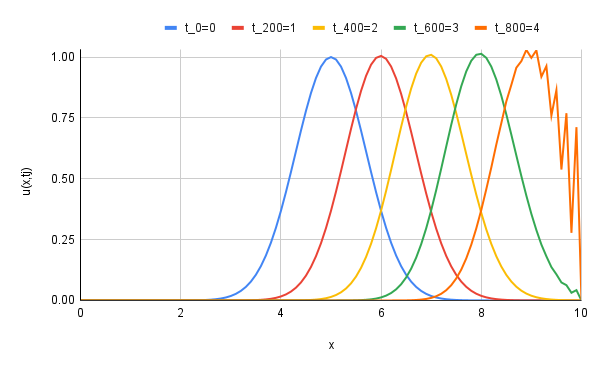
\includegraphics[width=0.85\textwidth]{0}
\end{figure}

dla nielepkiego równania Burgersa
\begin{equation}
\begin{split}
& \frac{1}{k}(u_{i,j+1}-u_{i,j})+\frac{1}{4h}(u_{i+1,j}^{2}-u_{i-1,j}^{2})=0\\
& u_{i,j+1}=u_{i,j}-\frac{k}{4h}(u_{i+1,j}^{2}-u_{i-1,j}^{2})
\end{split}
\end{equation}
\begin{figure}[h]
\caption{Nielepkie równanie Burgersa, metoda Eulera}
\centering
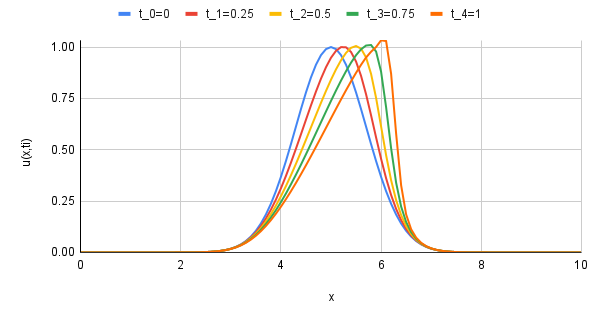
\includegraphics[width=0.85\textwidth]{1}
\end{figure}
\newpage

dla równania ciepła
\begin{equation}
\begin{split}
& \frac{1}{k}(u_{i,j+1}-u_{i,j})-\frac{\beta}{h^{2}}(u_{i+1,j}-2u_{i,j}+u_{i-1,j})=0\\
& u_{i,j+1}=u_{i,j}+\frac{\beta k}{h^{2}}(u_{i+1,j}-2u_{i,j}+u_{i-1,j})
\end{split}
\end{equation}
\begin{figure}[h]
\caption{Równanie ciepła, metoda Eulera}
\centering
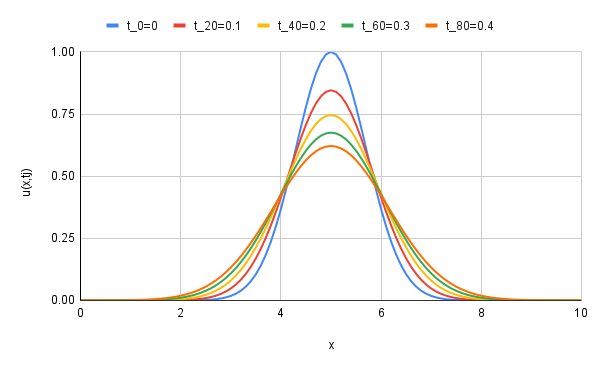
\includegraphics[width=0.85\textwidth]{2}
\end{figure}

dla równania Burgersa
\begin{equation}
\begin{split}
& \frac{1}{k}(u_{i,j+1}-u_{i,j})+\frac{1}{4h}(u_{i+1,j}^{2}-u_{i-1,j}^{2})-\frac{\beta}{h^{2}}(u_{i+1,j}-2u_{i,j}+u_{i-1,j})=0\\
& u_{i,j+1}=u_{i,j}-\frac{k}{4h}(u_{i+1,j}^{2}-u_{i-1,j}^{2})+\frac{\beta k}{h^{2}}(u_{i+1,j}-2u_{i,j}+u_{i-1,j})
\end{split}
\end{equation}
\begin{figure}[h]
\caption{Równanie Burgersa, metoda Eulera}
\centering
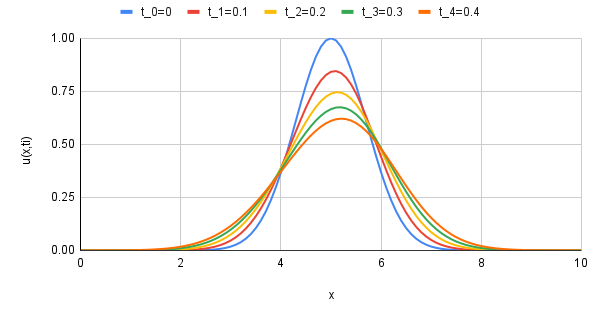
\includegraphics[width=0.85\textwidth]{3}
\end{figure}
\newpage

Stosując metodę Rungego-Kutty drugiego rzędu:\\
dla równania transportu
\begin{equation}
\begin{split}
& v_{i,j+1}=u_{i,j}-\frac{k}{4h}(u_{i+1,j}-u_{i-1,j})\\
& u_{i,j+1}=u_{i,j}-\frac{k}{2h}(v_{i+1,j+1}-v_{i-1,j+1})
\end{split}
\end{equation}
\begin{figure}[h]
\caption{Równanie transportu, metoda RK2}
\centering
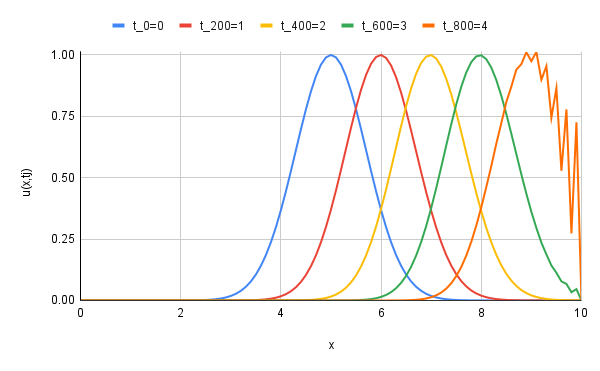
\includegraphics[width=0.85\textwidth]{4}
\end{figure}

dla nielepkiego równania Burgersa
\begin{equation}
\begin{split}
& v_{i,j+1}=u_{i,j}-\frac{k}{8h}(u_{i+1,j}^{2}-u_{i-1,j}^{2})\\
& u_{i,j+1}=u_{i,j}-\frac{k}{4h}(v_{i+1,j+1}^{2}-v_{i-1,j+1}^{2})
\end{split}
\end{equation}
\begin{figure}[h]
\caption{Nielepkie równanie Burgersa, metoda RK2}
\centering
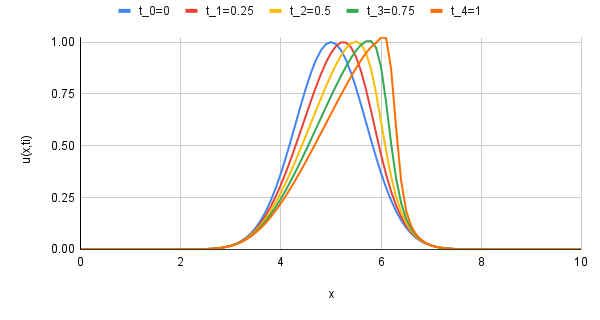
\includegraphics[width=0.85\textwidth]{5}
\end{figure}
\newpage
\newpage

dla równania ciepła
\begin{equation}
\begin{split}
& v_{i,j+1}=u_{i,j}+\frac{\beta k}{2h^{2}}(u_{i+1,j}-2u_{i,j}+u_{i-1,j})\\
& u_{i,j+1}=u_{i,j}+\frac{\beta k}{h^{2}}(v_{i+1,j+1}-2v_{i,j+1}+v_{i-1,j+1})
\end{split}
\end{equation}
\begin{figure}[h]
\caption{Równanie ciepła, metoda RK2}
\centering
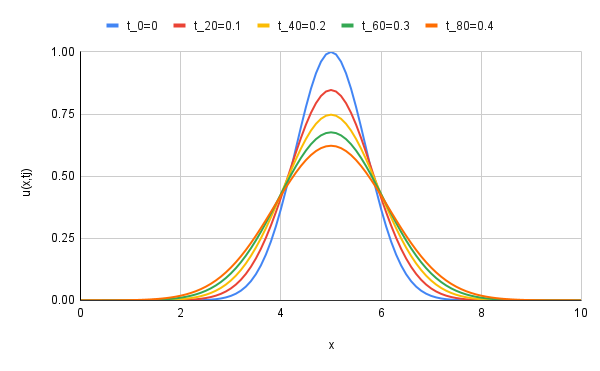
\includegraphics[width=0.85\textwidth]{6}
\end{figure}

dla równania Burgersa
\begin{equation}
\begin{split}
& v_{i,j+1}=u_{i,j}-\frac{k}{8h}(u_{i+1,j}^{2}-u_{i-1,j}^{2})+\frac{\beta k}{2h^{2}}(u_{i+1,j}-2u_{i,j}+u_{i-1,j})\\
& u_{i,j+1}=u_{i,j}-\frac{k}{4h}(v_{i+1,j+1}^{2}-v_{i-1,j+1}^{2})+\frac{\beta k}{h^{2}}(v_{i+1,j+1}-2v_{i,j+1}+v_{i-1,j+1})
\end{split}
\end{equation}
\begin{figure}[h]
\caption{Równanie Burgersa, metoda RK2}
\centering
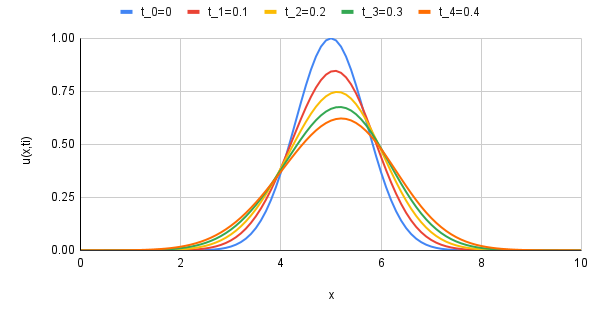
\includegraphics[width=0.85\textwidth]{7}
\end{figure}
\newpage

Stosując metodę niejawną:\\
dla równania ciepła
\begin{equation}
\begin{split}
& \frac{1}{k}(u_{i,j}-u_{i,j-1})-\frac{\beta}{h^{2}}(u_{i+1,j}-2u_{i,j}+u_{i-1,j})=0\\
& u_{i,j-1}=-\frac{\beta k}{h^{2}}u_{i-1,j}+(1+2\frac{\beta k}{h^{2}})u_{i,j}-\frac{\beta k}{h^{2}}u_{i+1,j}
\end{split}
\end{equation}
\begin{center}
$A=
\begin{bmatrix}
1+2s & -s & 0 & \cdots & 0\\
-s & 1+2s & -s & \cdots & 0\\
0 & -s & 1+2s & \cdots & 0\\
\cdots & \cdots & \cdots & \cdots & \cdots\\
0 & 0 & 0 & \cdots & 1+2s\\
\end{bmatrix}$
$, s=\frac{\beta k}{h^{2}}$
\end{center}
\begin{equation}
u_{i,j}=A^{-1}u_{i,j-1}
\end{equation}
\begin{figure}[h]
\caption{Równanie ciepła, metoda niejawna}
\centering
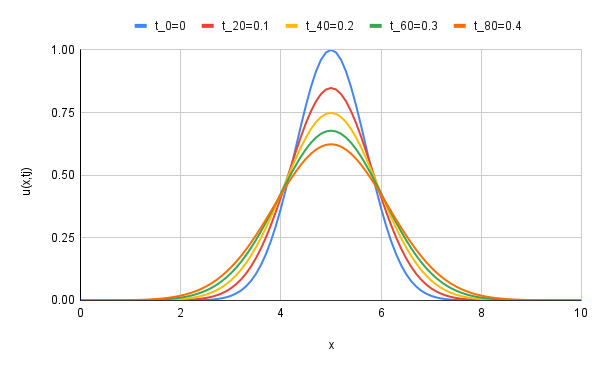
\includegraphics[width=0.85\textwidth]{8}
\end{figure}
\newpage

dla równania Burgersa
\begin{equation}
\begin{split}
& \frac{1}{k}(u_{i,j}-u_{i,j-1})+\frac{1}{4h}(u_{i+1,j-1}^{2}-u_{i-1,j-1}^{2})-\frac{\beta}{h^{2}}(u_{i+1,j}-2u_{i,j}+u_{i-1,j})=0\\
& u_{i,j-1}-\frac{k}{4h}(u_{i+1,j-1}^{2}-u_{i-1,j-1}^{2})=-\frac{\beta k}{h^{2}}u_{i-1,j}+(1+2\frac{\beta k}{h^{2}})u_{i,j}-\frac{\beta k}{h^{2}}u_{i+1,j}
\end{split}
\end{equation}
\begin{center}
$A=
\begin{bmatrix}
1+2s & -s & 0 & \cdots & 0\\
-s & 1+2s & -s & \cdots & 0\\
0 & -s & 1+2s & \cdots & 0\\
\cdots & \cdots & \cdots & \cdots & \cdots\\
0 & 0 & 0 & \cdots & 1+2s\\
\end{bmatrix}$
$,s=\frac{\beta k}{h^{2}}$
\end{center}
\begin{equation}
u_{i,j}=A^{-1}(u_{i,j-1}-\frac{k}{4h}(u_{i+1,j-1}^{2}-u_{i-1,j-1}^{2}))
\end{equation}
\begin{figure}[h]
\caption{Równanie Burgersa, metoda niejawna}
\centering
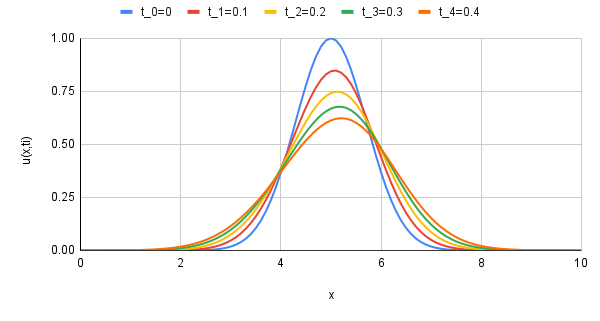
\includegraphics[width=0.85\textwidth]{9}
\end{figure}
\newline
Algorytm, który realizuje opisaną metodę niejawną korzysta z procedury tri rozwiązującej układ równań o macierzy trójprzekątniowej. Metoda tri korzysta ze szczególnego przypadku eliminacji Gaussa w czasie $O(n)$, zamiast czasu $O(n^3)$ dla normalnego przypadku, co ogromnie przyspiesza znajdowanie rozwiązań.
\newpage

Uzyskaliśmy prawie identyczne wyniki za pomocą użycia metody Eulera, RK2 i niejawnej. Nie mogliśmy skorzystać z metody niejawnej dla równania transportu, ani dla nielepkiego równania Burgersa, ponieważ wymaga ona użycia macierzy kwadratowej (M=N), a dla tych równań ta równość nie zachodziła.\\

Dla równania transportu oraz nielepkiego równania Burgersa, jeśli $t$ przekroczy odpowiednią wartość, to przybliżone wartości $u$ zaczynają bardzo mocno odbiegać od rzeczywistych (dla równania transportu $t>3$, dla nielepkiego równania Burgersa, $t>1$).\\

Dla równania transportu, kolejne przesunięcia w czasie powodują uzyskanie maksymalnej wartości $u$ w kolejnych przesunięciach w przestrzeni.  Funkcja Gaussa zostaje jedynie przesunięta w prawo.  Zobrazowna zostaje liniowość.\\

Dla nielepkiego równania Burgera, kolejne przesunięcia w czasie powodują uzyskanie maksymalnej wartości $u$ w kolejnych przesunięciach w przestrzeni. Funkcja Gaussa nie zostaje jedynie przesunięta w prawo, tylko wolniej rośnie przed osiągnieciem kresu i szybciej opada po osiągnięciu kresu. Zobrazowna zostaje nieliniowość.\\

Dla równania ciepła, kolejne przesunięcia w czasie powodują zmniejszenie kresu funkcji Gaussa. Maksymalna wartość $u$ maleje w tym samym punkcie w przestrzeni (5) dla kolejnych czasów.\\ 

Dla równania Burgersa, kolejne przesunięcia w czasie powodują zmniejszenie kresu funkcji Gaussa oraz powodują przesunięcie w prawo. Maksymalna wartość $u$ maleje i przesuwa się w przestrzeni dla kolejnych czasów.\\

Zwiększanie współczynnika $\beta$ powoduje zmniejszenie kresu $u(x,t)$. Dzieje się tak do około $\beta$ = 1.2, po czym rozwiązanie staje się całkowicie niepoprawne.\\
\begin{figure}[h]
\caption{Równanie Burgersa, metoda Eulera, $\beta$=1.3}
\centering
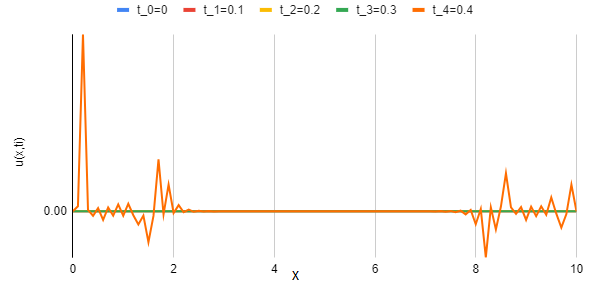
\includegraphics[width=0.85\textwidth]{10}
\end{figure}

Program komputerowy w języku C++ wyznaczający powyższe rozwiązania został dołączony w Dodatku A.
\end{document}